\PassOptionsToPackage{unicode}{hyperref}
\PassOptionsToPackage{aux}{rerunfilecheck}

\documentclass[aspectratio=1610]{beamer}

\usepackage{polyglossia}
\setmainlanguage{german}

\usepackage{amsmath}
\usepackage{amssymb}
\usepackage{mathtools}

\usefonttheme{professionalfonts}
\usepackage{fontspec}
\usepackage[
math-style=ISO,
bold-style=ISO,
nabla=upright,
partial=upright,
sans-style=italic,
]{unicode-math}
\setmathfont{Latin Modern Math}

\usepackage[
  math-micro=µ,
  locale=DE,
]{siunitx}

\usetheme{Frankfurt}
\usecolortheme{seagull}
\setbeamertemplate{navigation symbols}{}



% ImDokument:
% \author{...}
% \institute{...}
% \date{...}
% \title{...}

% \maketitle im ersten Frame
%\tableofcontents für ein Inhaltsverzeichnis


\usetheme{Warsaw}

%%% Fusszeile und deren Farbedefinitionen aus dem outertheme infolines
\setbeamercolor*{author in head/foot}{parent=palette tertiary}
\setbeamercolor*{title in head/foot}{parent=palette secondary}
\setbeamercolor*{date in head/foot}{parent=palette primary}
\makeatletter
\setbeamertemplate{footline}
{
  \leavevmode

  \hbox{

  \begin{beamercolorbox}[wd=.327\paperwidth,ht=2.25ex,dp=1ex,center]{author in head/foot}
    \usebeamerfont{author in head/foot}\insertshortauthor\expandafter\beamer@ifempty\expandafter{\beamer@shortinstitute}{}{~~(\insertshortinstitute)}
  \end{beamercolorbox}

  \begin{beamercolorbox}[wd=.327\paperwidth,ht=2.25ex,dp=1ex,center]{title in head/foot}
    \usebeamerfont{title in head/foot}\insertshorttitle
  \end{beamercolorbox}

  \begin{beamercolorbox}[wd=.327\paperwidth,ht=2.25ex,dp=1ex,right]{date in head/foot}
    \usebeamerfont{date in head/foot}\insertshortdate{}\hspace*{2em}
    \insertframenumber{} / \inserttotalframenumber\hspace*{2ex}
  \end{beamercolorbox}}

  \vskip0pt
}
\makeatother

%\usetheme{Singapore}
%\setbeamertemplate{sections/subsections in toc}[sections numbered]
%\setbeamertemplate{subsection in toc}[subsections numbered]

\author{Sebastian Pape \and Jonah Nitschke}
\institute{TU Dortmund}
\date{\today}
\title{Zusatzversuch: Die Wirbelstrombremse}
\subtitle{Anfängerpraktikum Physik III}


\begin{document}

\begin{frame}[plain]
  \titlepage
\end{frame}

\begin{frame}
  \frametitle{Inhaltsangabe}

  \begin{itemize}
    \item Theorie und Aufbau
    \item Durchführung
    \item Auswertung
    \item Diskussion
    \item Anwendungsbeispiele
    \item Fazit
    \item Quellen
  \end{itemize}

\end{frame}

\section{Theorie}

\begin{frame}
  \begin{figure}
    \centering
    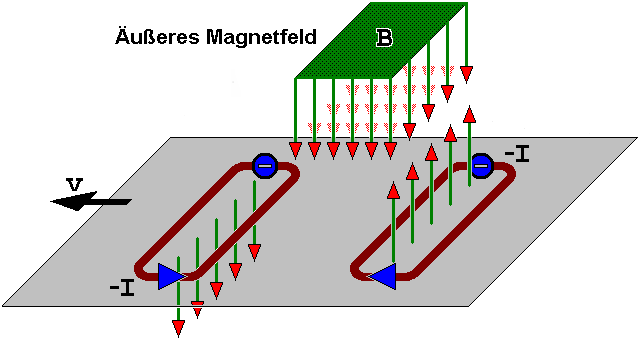
\includegraphics[width = \textwidth]{Lorentzkraft.png}
    \caption{Erzeugung von Wirbelströmen durch angelegtes äußere Magnetfeld. \cite{Lorentzkraft}}
  \end{figure}
\end{frame}

\section{Aufbau}

\begin{frame}

  \begin{columns}[onlytextwidth]
    \begin{column}{0.45\textwidth}
      \begin{figure}
        \centering
        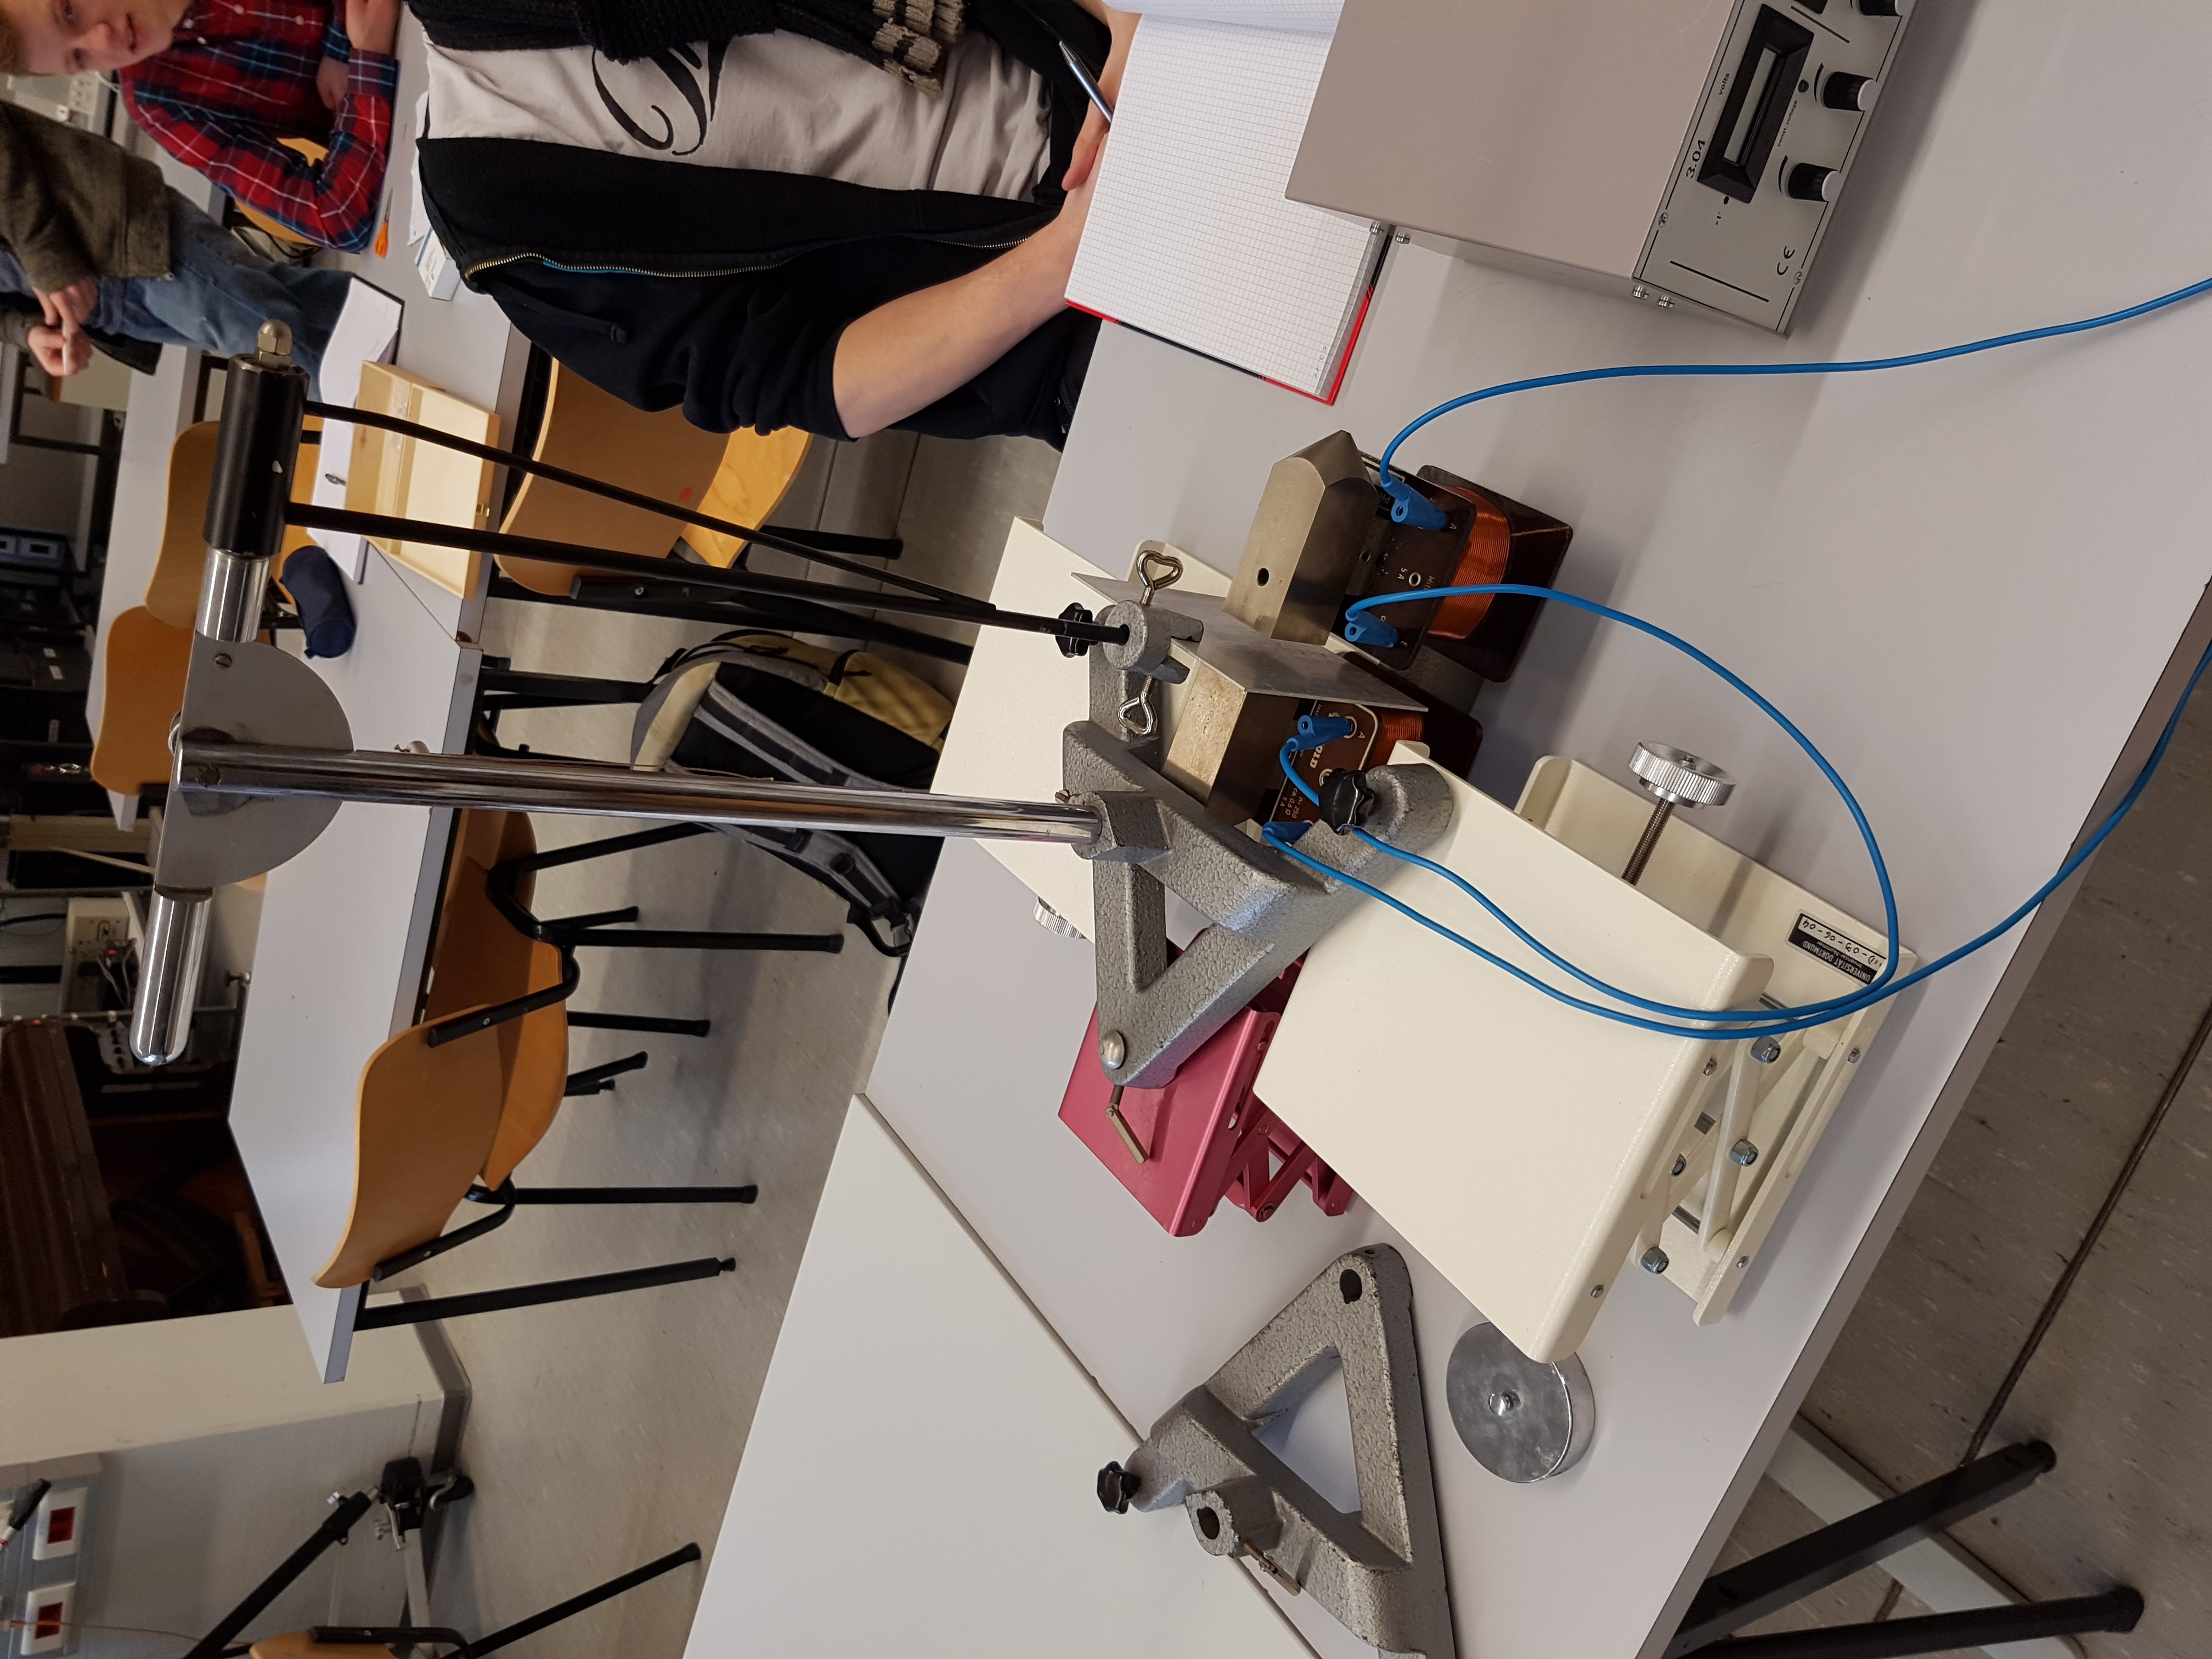
\includegraphics[height=5cm, angle = -90]{20170306_101228.jpg}
      \end{figure}
    \end{column}
    \begin{column}{0.45\textwidth}
      \begin{figure}
        \centering
        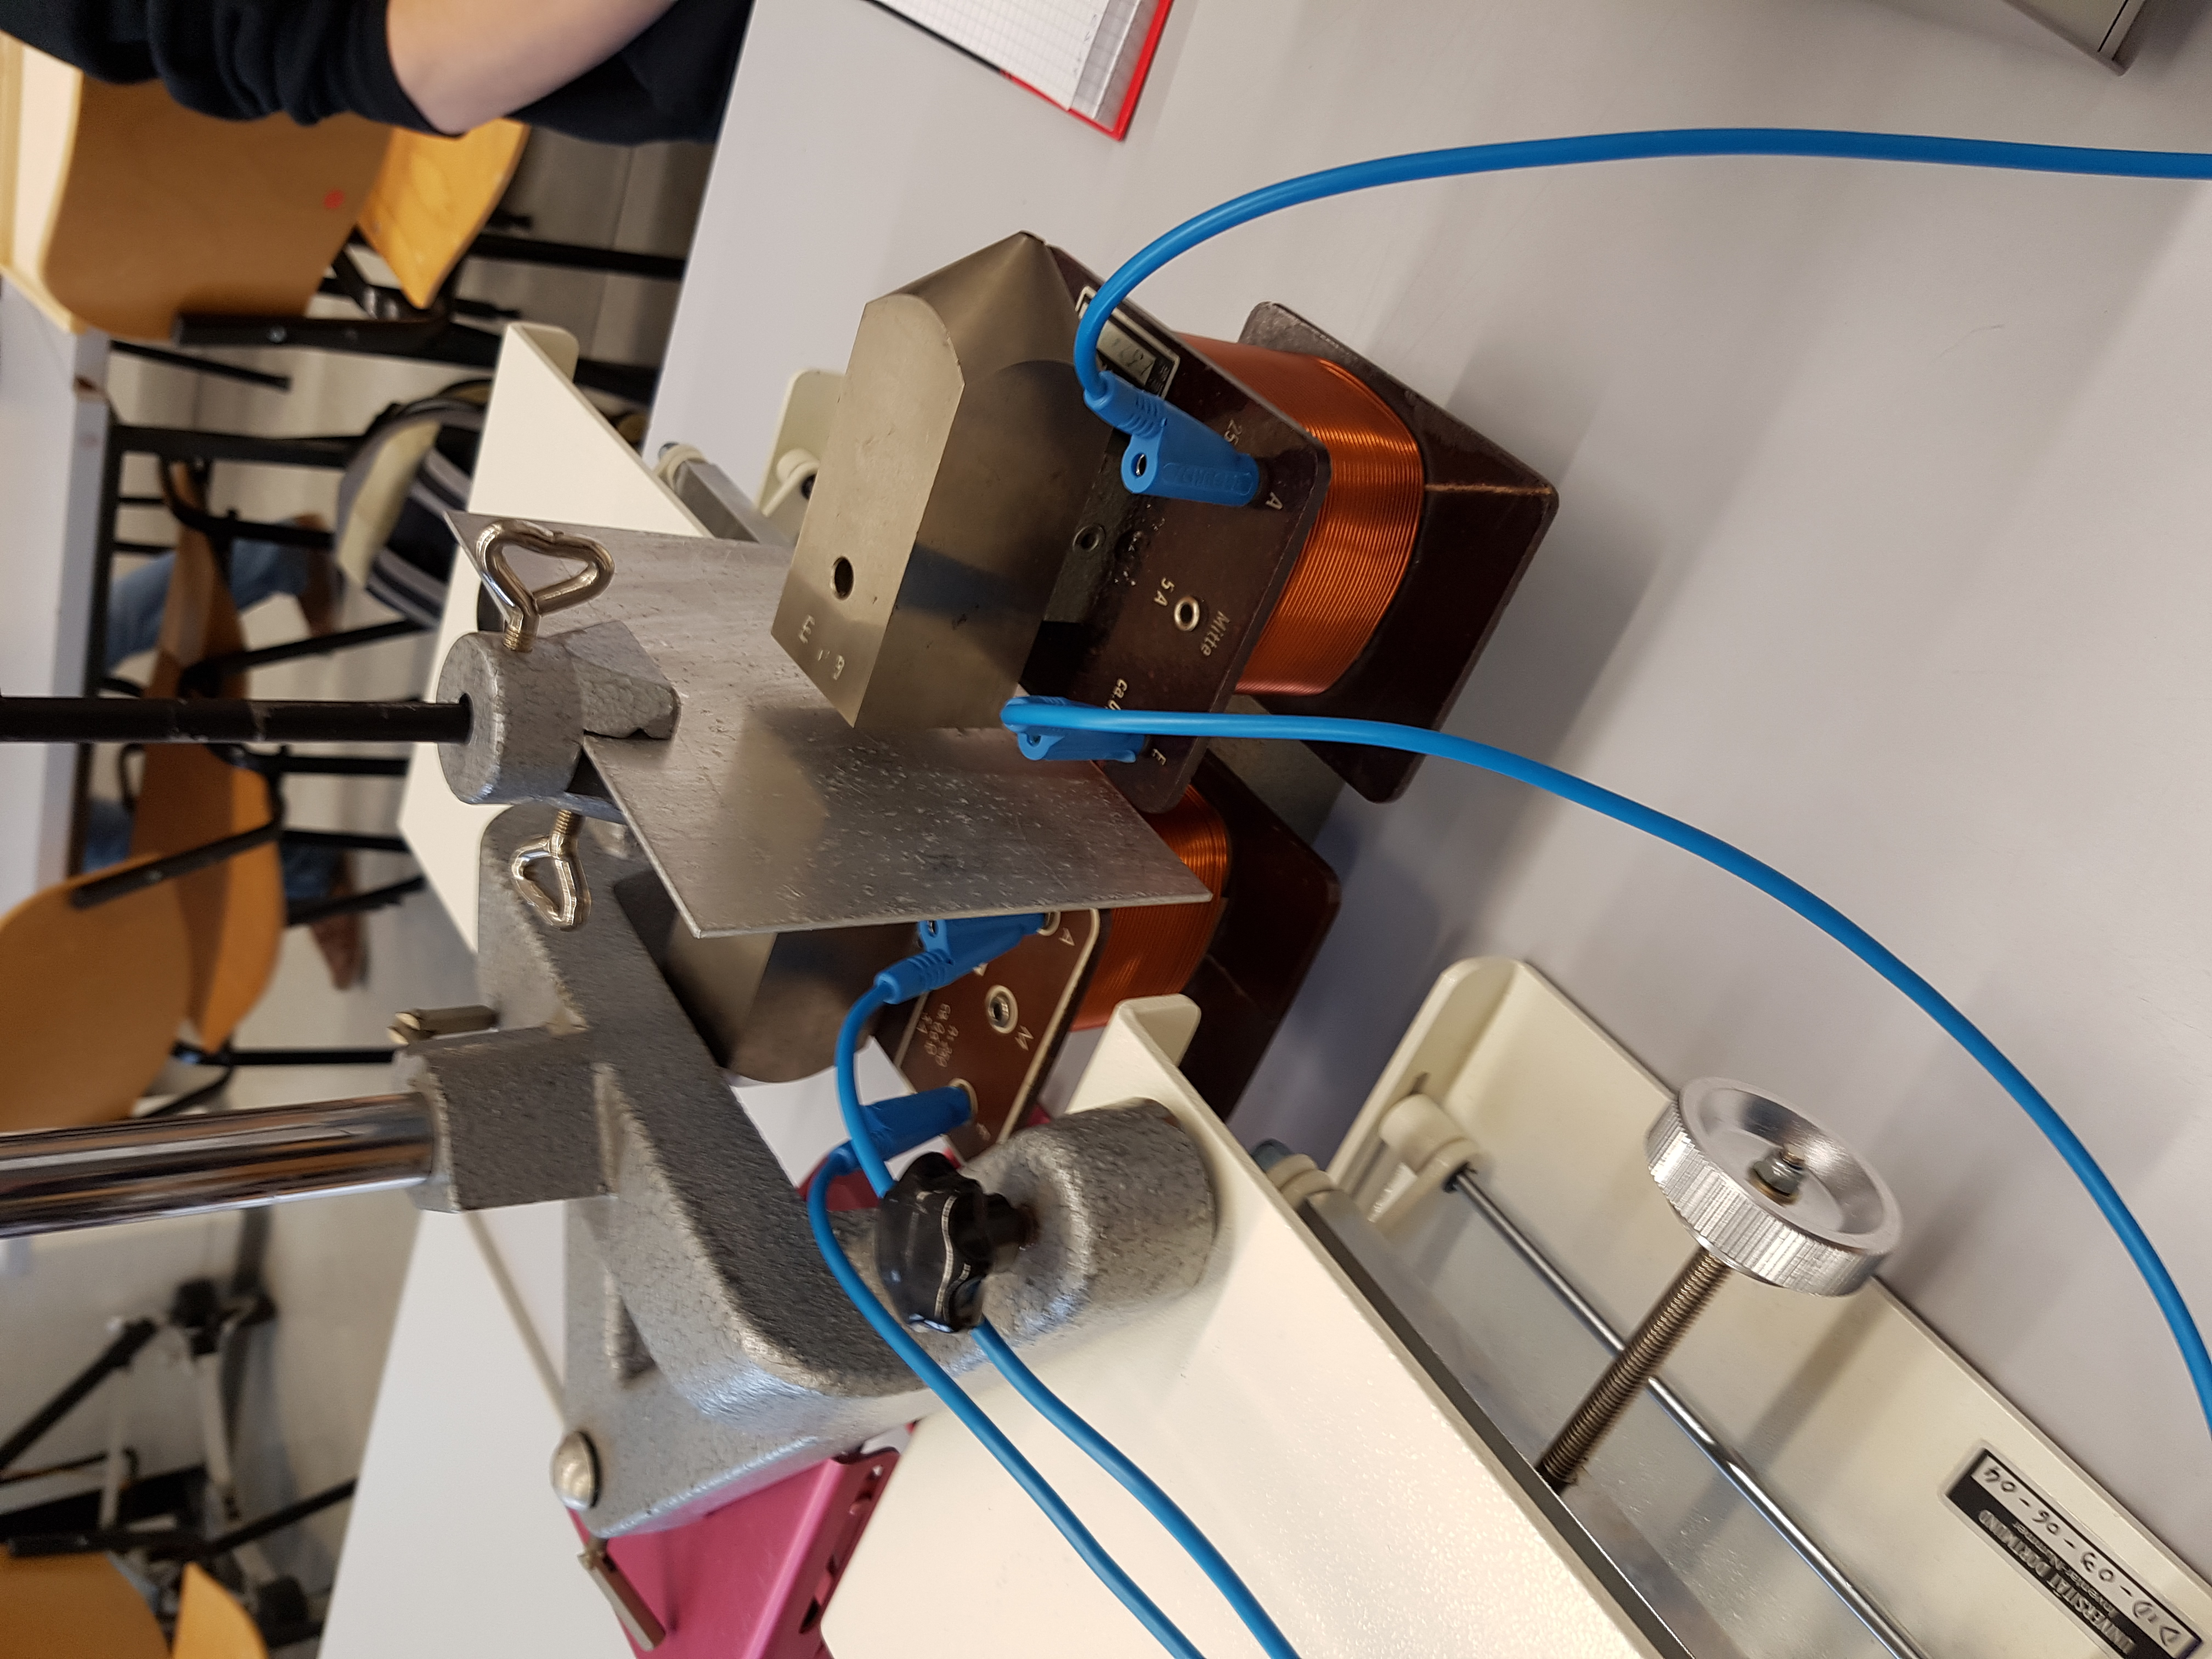
\includegraphics[height=5cm, angle = -90]{20170306_101230.jpg}
      \end{figure}
    \end{column}
  \end{columns}

\end{frame}

\section{Auswertung}

\begin{frame}
  \begin{figure}
    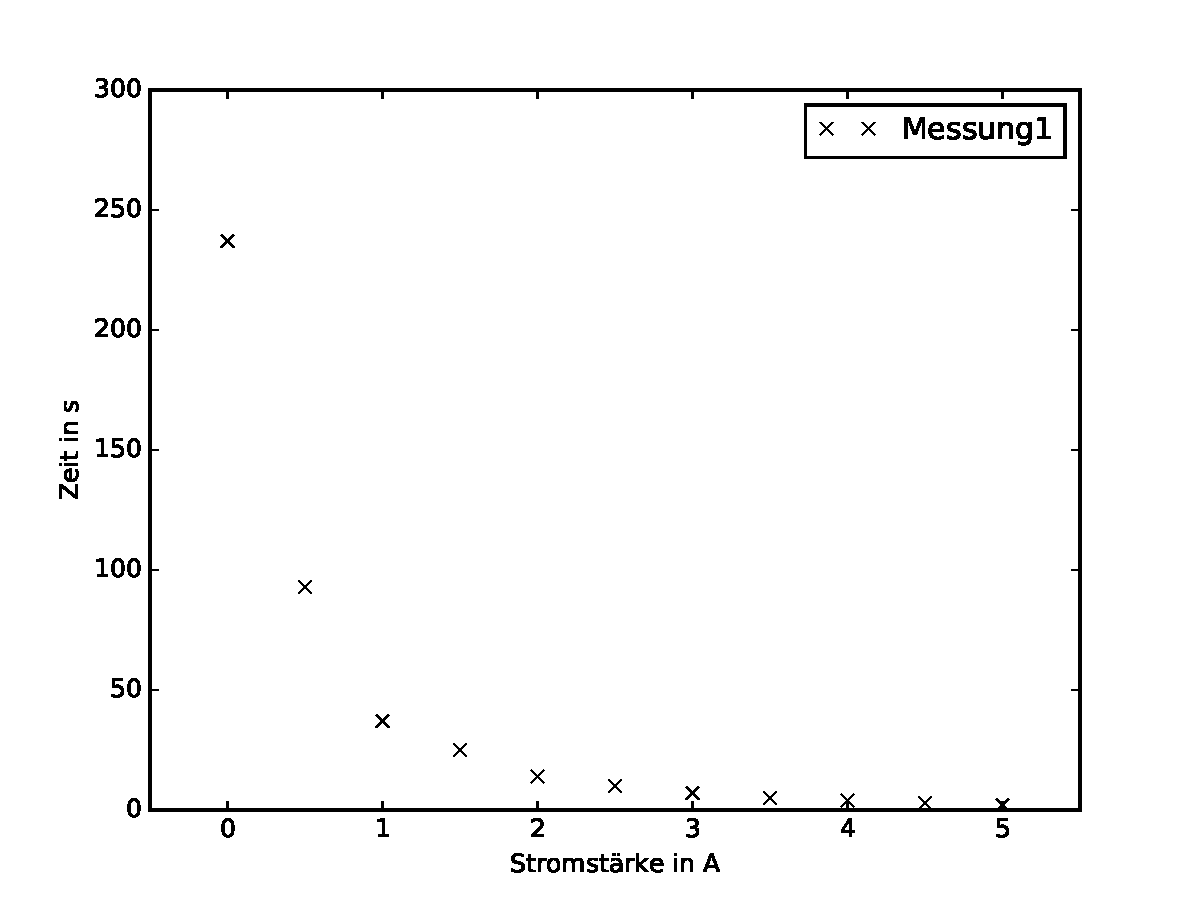
\includegraphics[width = 0.7\textwidth]{Messung1.pdf}
    \caption{Gemessene Zeiten in Abhängigkeit der angelegten Stromspannung bei einer ungeschlitzten Platte.}
  \end{figure}
\end{frame}

\begin{frame}
  \begin{figure}
    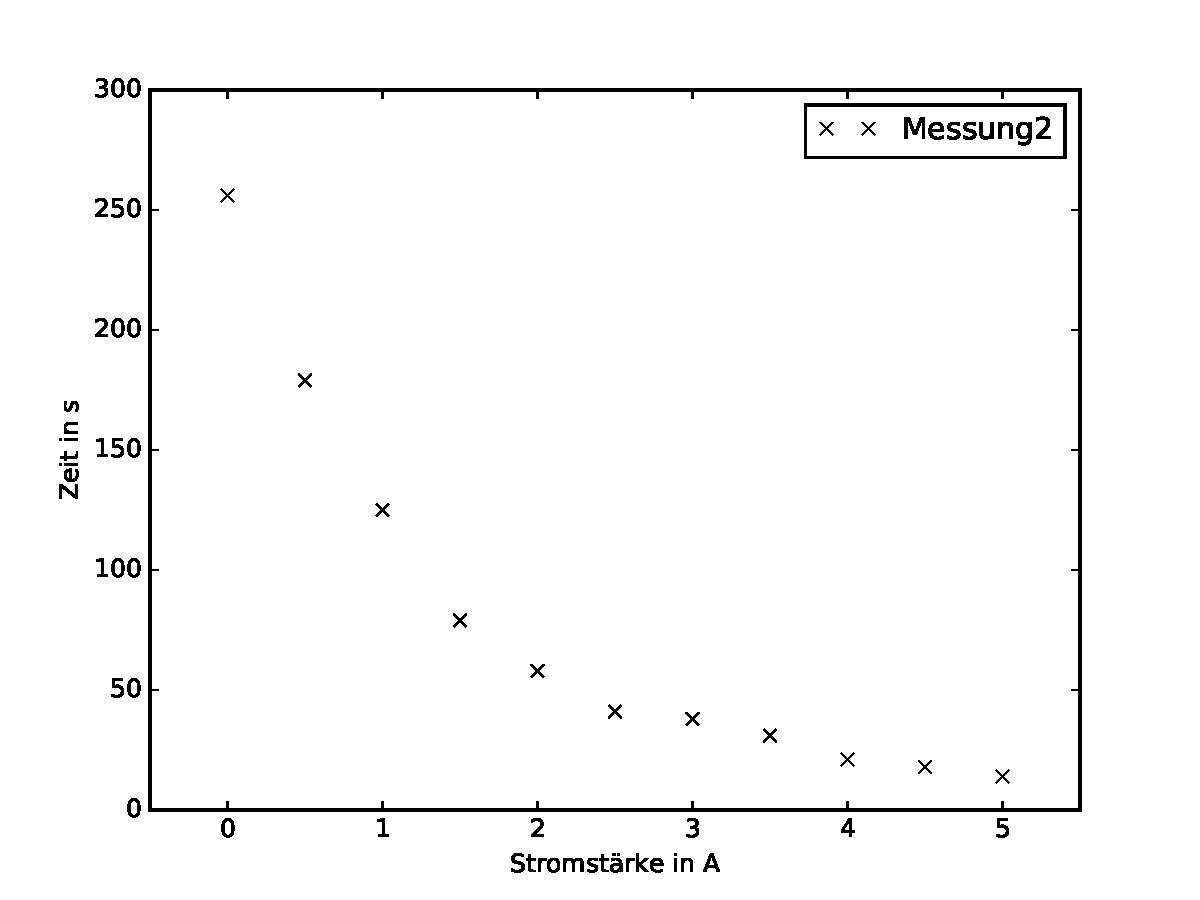
\includegraphics[width = 0.7\textwidth]{Messung2.pdf}
    \caption{Gemessene Zeiten in Abhängigkeit der angelegten Stromspannung bei einer leicht geschlitzten Platte.}
  \end{figure}
\end{frame}

\begin{frame}
  \begin{figure}
    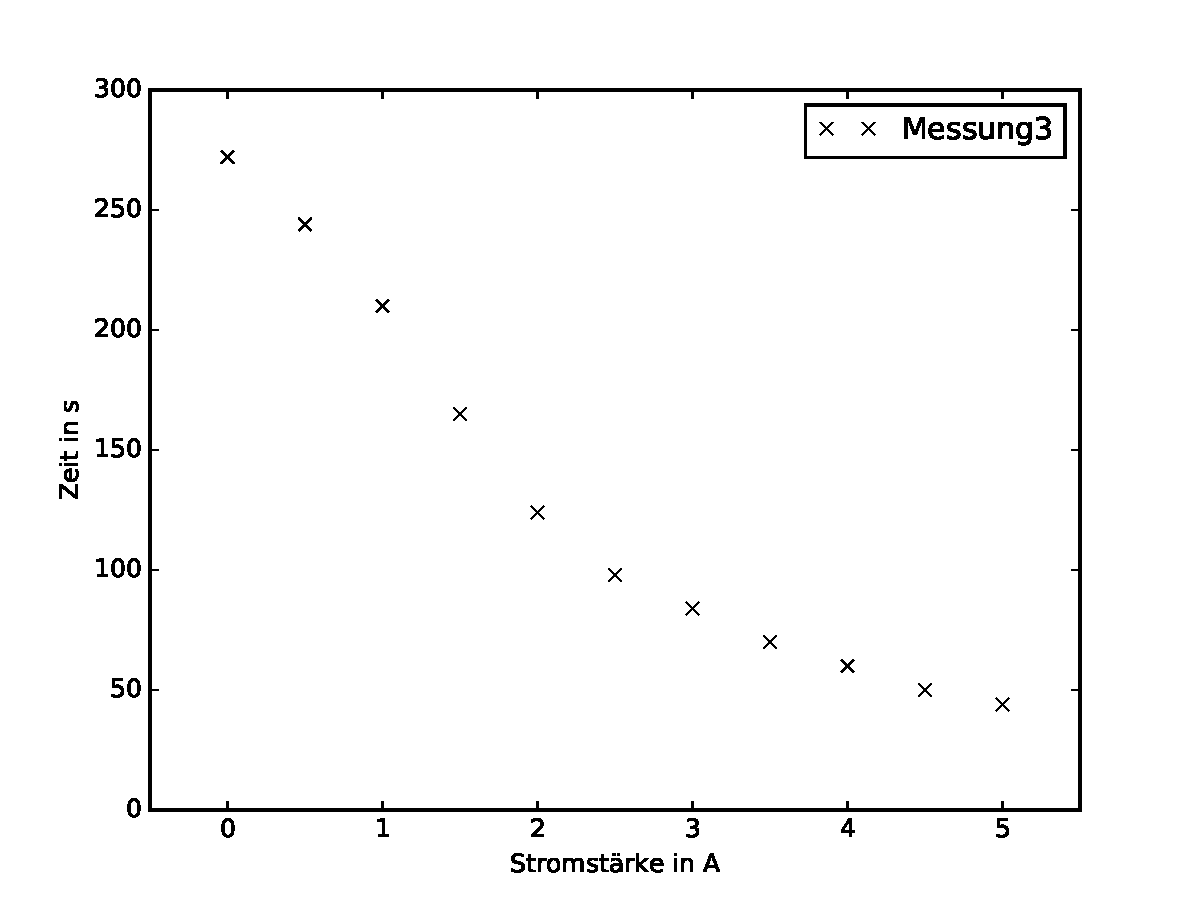
\includegraphics[width = 0.7\textwidth]{Messung3.pdf}
    \caption{Gemessene Zeiten in Abhängigkeit der angelegten Stromspannung bei stark geschlitzten Platte.}
  \end{figure}
\end{frame}

\begin{frame}
  \begin{figure}
    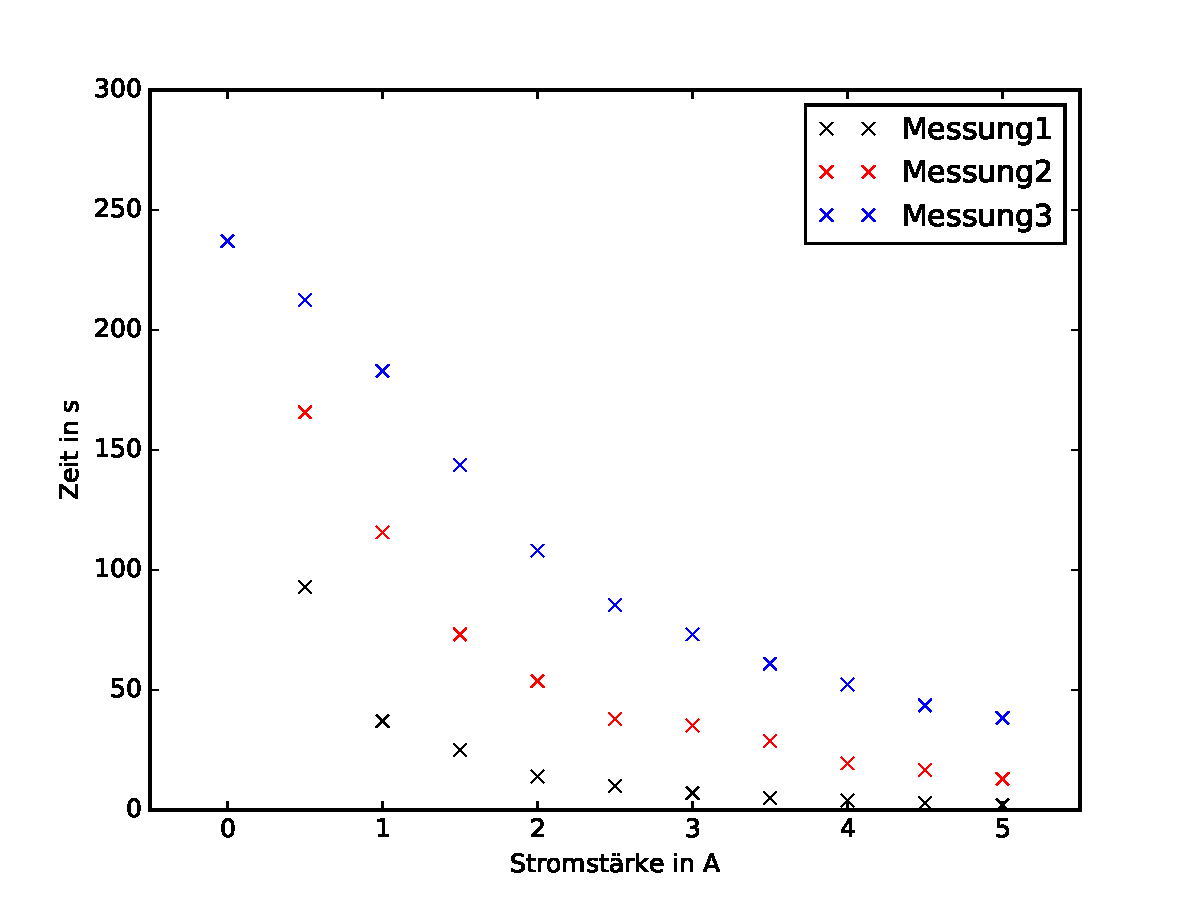
\includegraphics[width = 0.7\textwidth]{Kombiniert_gestaucht.pdf}
    \caption{Prozentuale Dämpfung in Abhängigkeit der angelegten Stromspannung.}
  \end{figure}
\end{frame}

\begin{frame}

  \begin{table}
    \caption{Auftretende Dämpfung bei den verschiedenen Platten}
     \begin{tabular}{c c c}
        \toprule
        Anz. Einkerbungen & Dämpfung in $\%$ & Fehler \\
        \midrule
        0 & 0.84 & 0.21 \\
        6 & 5.47 & 0.20 \\
        12 & 16.18 & 0.19 \\
        \bottomrule
      \end{tabular}
  \end{table}

\end{frame}

\section{Anwendungsbeispiel}

\begin{frame}
  \begin{figure}
    \centering
    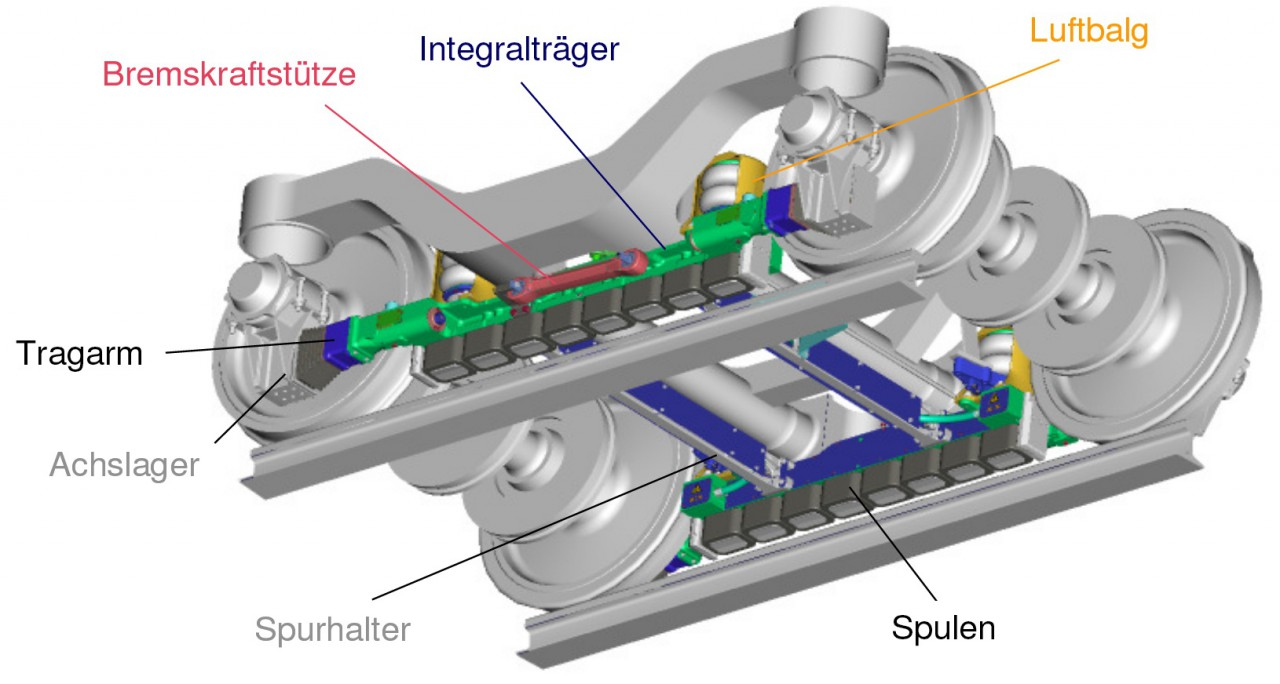
\includegraphics[width=0.7\textwidth]{Wirbelstrombremse_Aufbau.jpg}
    \caption{Aufbau einer linearen Wirbelstrombremse. \cite{Wirbelstrombremse}}
    \label{fig:linWAufbau}
  \end{figure}
\end{frame}

\section{Fazit}

\begin{frame}
  \centering
  \Huge Fazit
\end{frame}


\begin{frame}
  \printbibliography
\end{frame}


\end{document}
